\documentclass[czech,bachelor]{diploma}

\usepackage[autostyle=true,czech=quotes]{csquotes} % korektni sazba uvozovek, podpora pro balik biblatex
\usepackage[backend=biber, style=iso-numeric, alldates=iso]{biblatex} % bibliografie
\usepackage{dcolumn} % sloupce tabulky s ciselnymi hodnotami
\usepackage{subfig} % makra pro "podobrazky" a "podtabulky"

\usepackage{float} % lepsi umistovani obrazku (H)

% Pozadovane vstupy pro generovani titulnich stran.
\ThesisAuthor{Barbora Kovalská}
\ThesisSupervisor{doc. Ing. Radoslav Fasuga, Ph.D.}

\CzechThesisTitle{Tvorba herního modelu výpravné evoluční hry}
\EnglishThesisTitle{Creation of the Game Model for the Narrative Evolution Game}

\SubmissionYear{2024}

\ThesisAssignmentFileName{../specification.pdf}

\Acknowledgement{Ráda bych nepoděkovala svému minulému já za to, že se rozhodla na práci nepracovat.}

\CzechAbstract{Tato bakalářská práce se zabírá vytvořením a dokumentací herního systému pro hybridní deskovou hru.}
\CzechKeywords{desková hra; herní design}

\EnglishAbstract{This bachelor's thesis deals with the creation and documentation of a game system for a hybrid board game.}
\EnglishKeywords{board game; game design}

\AddAcronym{TTS}{Trails Through Shadows}
\AddAcronym{RPG}{Role Playing Game}
\AddAcronym{D\&D}{Dungeons \& Dragons}

\addbibresource{Resources/websites.bib}

% Novy druh tabulkoveho sloupce, ve kterem jsou cisla zarovnana podle desetinne carky
\newcolumntype{d}[1]{D{,}{,}{#1}}

% Uprava hloubky obsahu - pozdeji smazat !
\setcounter{tocdepth}{2}


% Zacatek dokumentu
\begin{document}

% Titulni strany
\MakeTitlePages

% Seznam obrazku
\listoffigures
\clearpage

% Seznam tabulek
\listoftables
\clearpage

% Text zaverecne prace.
\chapter{Úvod}

Welcome to hell. This is the introduction chapter.

\chapter{Historie a základní pojmy}
\label{chap:theory}

V této kapitole si ve zkratce popíšeme historii deskových her, zmíníme některé důležité tituly a představíme základní pojmy herní teorie a designu.


\section{Historický vývoj}
\label{sec:history}

Deskové hry lidstvo provázejí už překvapivě dlouhou dobu. Ať už sloužily jako zábava, nástroj ke vzdělávání nebo jen jako aktivita umožňující sociální kontakt, vždy byly součástí lidské kultury. Vývoj deskových her odráží vývoj lidské civilizace - změny v technologiích, kultuře a filozofii. V následujících sekcích si přiblížíme historii, kterou si deskové hry v průběhu času prošly.

\subsection{Počátky}
\label{subsec:beginnings}

Za úplně první deskové hry bychom mohli považovat kostky. Ty byly nalezeny v různých prehistorických nalezištích, což znamená, že lidstvo si s nimi hrálo dřív, než začalo zanechávat písemné záznamy. Kromě kostek se však našly i jiné předměty, které byly pravděpodobně používány k hraní her. Šlo například o sadu barevných vyřezávaných kamínků, které byly nalezeny v Turecku, nebo zdobená dřívka z Mezopotámie. \cite{attia_2018}

Nejstarší deskovou hrou, kterou známe, je hra jménem \textit{The Royal Game of Ur}, pocházející z Mezopotámie. Byla objevena v hrobce krále Ur, který žil před 4500 lety. Hra byla pro dva hráče, kteří měli za úkol jako první dopravit své figurky na konec herního pole. Zajímavé také je, že se spolu s hrou uchovala i její pravidla, napsaná v klínovém písmu na destičky. Mezi další hry z této doby patří například \textit{Senet}, která byla oblíbená v Egyptě, nebo \textit{Mahjong}, která pochází z Číny. \cite{british_museum_2021}

\begin{figure}[H]
    \centering
    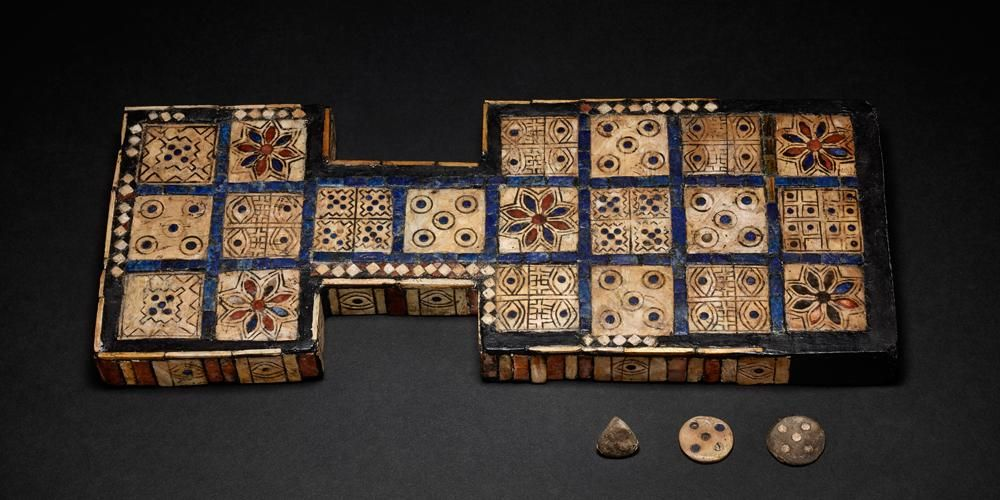
\includegraphics[width=0.7\textwidth]{Figures/Theory/royal-game-of-ur-british-museum.jpg}
    \caption{Replika hry \textit{The Royal Game of Ur} v British Museum. \cite{british_museum_2021}}
    \label{fig:royal_game_of_ur}
\end{figure}

Dále by se do této kategorie daly zařadit i velmi oblíbené \textbf{Šachy}, které zdánlivě provází lidstvo už od počátků. Jejich historie sahá do roku 400 př. n. l., kdy vznikla keltická hra \textit{Tafl}. Jednalo se o asymetrickou hru, ve které se jeden hráč snažil utéct se svým králem, začínajícím hru ve středu šachovnice, zatímco druhý hráč se snažil krále chytit. Historici se domnívají, že tato verze byla v Indii 6. století našeho letopočtu převzata a pozměněna ve hru \textit{Chaturanga}. Během let její popularita rostla a rozšířila se do celé Asie a nakonec i do Evropy. Do formy, kterou známe dnes, se šachy dostaly právě v Evropě až v 16. století. \cite{chess_com_2023}

Už takhle brzy tedy můžeme zaznamenat dodnes využívané herní principy: herní pole složené z políček, po kterých se hráči pohybují podle hodů kostkou, a cíl hry, kterým je dosažení určitého cíle na herním poli. \cite{attia_2018}

\subsection{Vývoj deskových her}
\label{subsec:development}

V období od 18. století se deskové hry stávaly více populárnějšími, s čímž se také zvedal zájem o jejich vývoj. Hry byly komplexnější a jejich tvorba se stala výdělečným odvětvím.

Jako jedna z prvních vývojářek deskových her je považována Američanka Elizabeth Magie, která v roce 1903 vytvořila hru \textit{The Landlord's Game}. Hra byla zamýšlena jako nástroj k vzdělávání a varování proti riskům land grabbingu - tedy spekulací s pozemky. Hráči se v ní snažili koupit pozemky, stavět na nich domy a hotely a tím získávat od ostatních hráčů peníze. V roce 1935 Magie prodala patent na hru společnosti Parker Brothers za 500 dolarů. Ti hru přejmenovali na \textbf{Monopoly} a začali ji prodávat, což se ukázalo být velmi úspěšné. \cite{attia_2018}

\begin{figure}[H]
    \centering
    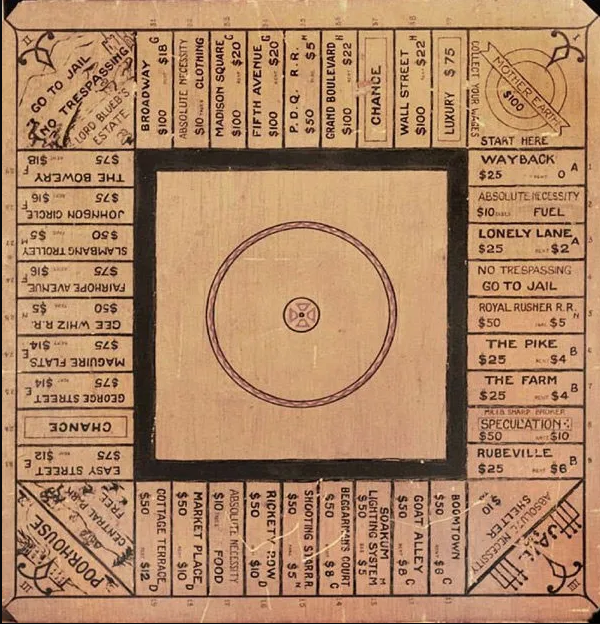
\includegraphics[width=0.3\textwidth]{Figures/Theory/landlords-game.png}
    \caption{Hra \textit{The Landlord's Game} od Elizabeth Magie. \cite{attia_2018}}
    \label{fig:landlords-game}
\end{figure}

V německu se deskové hry rozrostly tak moc, že se zde vytvořila vlastní kultura deskových her. V roce 1978 byla založena společnost \textit{Spiel des Jahres}, která každý rok uděluje cenu pro nejlepší hru roku. Tato cena se stala velmi prestižní a zvýšila zájem o deskové hry po celém světě. Zapříčinila se například za úspěch her jako \textit{Osadníci z Katanu} nebo \textit{Dixit}. \cite{attia_2018}

\subsection{Moderní směr}
\label{subsec:modern}

Kvůli vzniku a úspěchu spousty dalších her, například \textit{Carcassonne}, \textit{Ticket to Ride} nebo \textit{Risk}, se čím dál více lidí chtělo stát jejich vývojáři. V tomto jim pomohl jeden z dalších milníků - vznik Kickstarteru. Tato platforma umožňuje vývojářům prezentovat své nápady a získat na ně finanční podporu od lidí, kteří by je chtěli vidět na trhu.  \cite{attia_2018}

Díky tomu deskové hry prošly další revolucí, neboť teď tu byla možnost propagovat hru přímo hráčům, kteří by ji chtěli hrát. Velmi úspěšné projekty jako \textit{Exploding Kittens} nebo \textit{Gloomhaven} získaly na Kickstarteru miliony dolarů. Také zde začaly vznikat deskové implementace existujících videoherních titulů, jako například \textit{Darkest Dungeon: The Board Game}, \textit{The Witcher: Old World} nebo \textit{Dark Souls - The Board Game}. \cite{kickstarter}

Nemůžeme zapomenout zmínit ani giganta mezi deskovými hrami, který přinesl revoluci v herním designu - \textbf{Dungeons \& Dragons}. Tato hra, vytvořená Gary Gygaxem a Davidem Arnesonem, byla první stolní hrou, která se zaměřovala na příběh a roleplay. Hráči si v ní vytvářeli své postavy a procházeli s nimi dobrodružstvím, které jim připravoval tzv. \textit{Dungeon Master} - hráč, který hru řídil a vytvářel pro ostatní dobrodruhy příběh. Tento nápad byl tak úspěšný, že vytvořil celý žánr - \textit{tabletop RPGs} - a inspiroval spoustu dalších her, jak deskových, tak videoherních. \cite{dnd_beyond_2023}

V moderních hrách můžeme pozorovat, že se stále více zaměřují na roleplay a příběh a hlouběji implementují RPG prvky. I herní mechanismy se stávají více komplexními a vývojáři se nebojí experimentovat s novými nápady. Hry začínají být i obsáhlejší, což se projevuje v delší době hraní, větší složitosti pravidel a větším množství fyzických komponent.


\section{Definice pojmu desková a stolní hra}
\label{subsec:boardgame_definition}

V této oblasti herního designu se můžeme setkat se dvěma základními pojmy: \textit{desková hra} a \textit{stolní hra}. Tyto pojmy se často používají zaměnitelně, ale mají odlišné významy. Proto si je zde přiblížíme.

\textbf{Desková hra} (board game) je obvykle hra, jejíž hlavní součástí a neoddělitelnou komponentou je herní deska. Samotné provedení desky se může lišit, může se jednat o klasickou čtvercovou desku, nebo o jiný tvar, jako například kruhovou, hexagonální nebo jinou. Deska může být také rozdělena na políčka, která mohou mít různé vlastnosti, například barvu, číslo nebo symbol. Hra může mít také další komponenty, jako jsou karty, kostky, figurky, žetony, atd. Herní systém většinou bývá intuitivní a jednoduchý, snažící se zaměřit na širší publikum hráčů. Herní mechaniky se často točí okolo desky a ostatních fyzických komponent a neobsahují velkou míru abstrakce. Do této kategorie patří například \textit{Monopoly}, \textit{Osadníci z Katanu} nebo \textit{Carcassonne}. \cite{board_game_supply_2023}

\textbf{Stolní hra} (tabletop game) je obecnější termín, který zahrnuje všechny hry, které se hrají na stole. To znamená, že do této kategorie můžeme zařadit i hry, které nemají herní desku, jako například karetní hry, hry s kostkami, nebo hry, které se hrají pouze s papírem a tužkou. I když jsou komponenty jejich důležitou součástí, některé stolní hry si dovolují vyšší míru abstrakce herních systémů, což jim dává větší možnosti hloubky na úkor odcizení některých skupin hráčů. Toto můžeme pozorovat například u prosperujícího žánru RPG her, kam můžeme zařadit Na vlnách neznáma, \textit{Gloomhaven} nebo i výše zmíněné \textit{Dungeons \& Dragons}. \cite{board_game_supply_2023}

Pro účely této práce se budeme věnovat především deskovým hrám, ale budeme se snažit zahrnout i některé prvky stolních her, které by mohly být pro náš návrh užitečné.
\chapter{Teorie herního designu}
\label{chap:game_design}

V této kapitole jsou popsány základní pojmy herní teorie a designu, které budou sloužit jako základ pro vlastní návrh. \cite{building_blocks_of_tabletop_design_2022}


%%% section: Structure %%%

\section{Herní struktura}
\label{sec:structure}

Herní struktura je základním stavebním kamenem každé hry. Jedná se o sadu pravidel, která určují, jak se hraje, co mohou hráči dělat a jakým způsobem se hra vyhrává. Typy struktur se liší podle jejich přístupu k herním systémům a mechanikám. 

\subsection{Kompetetivní hry}
\label{subsec:structure_competitive}

Kompetetivní hry tvoří velkou část trhu s deskovými hrami. V těchto hrách se hráči snaží porazit ostatní a dosáhnout vítězství. Tyto hry můžou být symetrické, kdy všichni hráči začínají se stejnou nebo alespoň podobnou silou, nebo asymetrické, kdy mají hráči různé schopnosti a cíle. Častým problémem bývá vybalancovat hru tak, aby byla zábavná pro všechny hráče, a to i přesto, že se může stát, že jeden hráč bude mít výhodu. Dále se často stává, že hra skončí remízou. V takovém případě se může o vítězi rozhodnout buď pomocí nějakých dodatečných pravidel, nebo může skončit sdíleným vítězstvím.

Příklady: \glsref{monopoly}, \glsref{carcassonne}, \glsref{chess}, \glsref{race_for_the_galaxy}

\subsection{Kooperativní hry}
\label{subsec:structure_cooperative}

Naopak kooperativní hry se snaží hráče spojit proti společnému nepříteli nebo problému. Hráči spolupracují na dosažení cíle, který je obvykle nějakým způsobem předem daný. Velkou výhodou toho typu her je to, že odstraňují překážky, které by lidem bránily si tento typ her zahrát. Když jsou hráči spolu ve stejném týmu, dokáží vyrovnat jejich schopnosti a zkušenosti, což může novým hráčům pomoci se do hry dostat.

Kooperativní hry se dají dále rozdělovat podle různých kritérií. Například některé mohou hráče spojit v boji proti oponentovi ve formě umělé inteligence nebo sady algoritmů, zatímco jiné dávají týmu za úkol vyřešit hádanku a nemají žádného protivníka. Dalším kritériem může být, jestli hra má skryté informace, nebo jestli jsou všechny informace sdílené. Sdílení zdrojů, způsob komunikace a způsob, jakým se hra vyhrává, jsou dalšími faktory, které mohou kooperativní hru ovlivnit.

Příklady: \glsref{pandemic}, \glsref{arkham_horror}, \glsref{gloomhaven}, \glsref{forgotten_waters}


\subsection{Hry se scénářem}
\label{subsec:structure_scenario}

Tento typ her se často zaměřuje především na příběh, historickou tematiku a RPG elementy. Průběh hrou se skládá z jednotlivých epizod, které můžou být předem naplánované a navázané na sebe. Tento systém se často používá v tzv. \textit{dungeon crawlerech}, kde hráči prochází jeden dungeon za druhým. S tímto formátem je jednoduché vyměnit mapu, typy nepřátel nebo příběhové zabarvení a hráči mohou zažít více dobrodružství bez toho, aby se museli učit nová pravidla. Je to také jednoduchý způsob, jak nastavit obtížnost hry, protože každý scénář může být jiný.

Příklady: \glsref{catan}, \glsref{gloomhaven}, \glsref{pathfinder}

\subsection{Legacy hry}
\label{subsec:structure_legacy}

Legacy hry jsou speciální typ her, který se vyznačuje nenávratnými změnami, které hráči během hraní páchají na herních komponentách. Jde o změny fyzického rázu, jako je psaní na herní desku, trhání karet nebo lepení nálepek. Tyto změny mohou být způsobeny výsledkem hry, nebo mohou být součástí příběhu. Tento typ her se často zaměřuje na příběh a vývoj postav, a proto mají velmi blízko k RPG žánru. Kampaně v nich mohou trvat i několik měsíců či let, rozdělených do jednotlivých několikahodinových sezení. Jedná se o relativně nový fenomén, který se však v posledních letech začal rozšiřovat a získal si své publikum.

Příklady: \glsref{risk_legacy}, \glsref{hp_hogwarts_battle}, \glsref{gloomhaven}


%%% section: Turns %%%

\section{Pořadí a struktura tahů}
\label{sec:turns}

Se zavedením struktury přichází potřeba rozhodovat, kdy hráči mohou konat různé akce nebo kroky. Odsud vznikla myšlenka \textbf{tahu} - jednotky času, během které mohou hráči se hrou interagovat. Více tahů pak tvoří jedno \textbf{kolo}, přičemž běžné hry se skládají z několika takovýchto kol. V některých titulech se kola navíc rozdělují do několika \textbf{fází}, které většinou třídí akce do různých typů, čímž umožňují ještě větší stukturovanost herního kola. Tato pravidla se však mohou lišit podle typu hry, proto se tato sekce věnuje přiblížení několika základních typů struktury tahů.

\subsection{Kolo s pevným pořadím}
\label{subsec:turns_fixed_order}

Jedná se o nejzákladnější typ struktury kola, kdy se pořadí hráčů určí jednou na začátku hry a od té doby zůstává neměnné. Obvykle se nějakým způsobem vybere první hráč a dál tahy pokračují podél stolu ve směru nebo proti směru hodinových ručiček (například v klasické karetní hře \textit{Prší}). Tento typ struktury je velmi jednoduchý a intuitivní, ale může být nevýhodný pro hry, kde je výhoda mít první tah, nebo chceme zajistit, aby všichni hráči měli stejný počet tahů. Toto se dá řešit zvýhodněním odstaních hráčů jinými způsoby, například herními bonusy (mana navíc pro druhého hráče v \glsref{hearthstone}), nebo tím, že budeme monitorovat, který hráč začínal, a poslední kolo se vždy dojede až k němu, i kdyby hra byla ukončena v průběhu kola (jako v \glsref{through_the_ages}, kde všichni dojedou celé kolo po tom, co jeden hráč zvítězí).

\subsection{Kolo s pořadím podle statistik}
\label{subsec:turns_stat_order}

Tento typ struktury kola se snaží vyrovnat výhody a nevýhody, které mohou vzniknout z pevného pořadí. Pořadí se v tomto případě mění podle nějakého skóre, které se během hry mění. Určující statistikou může být například počet bodů, které hráči mají (tokeny populace v \glsref{civilization}), nebo nějaké pevnější statistiky spojené se samotnými postavami. Tento systém se často používá v RPG hrách, kde se pořadí může měnit podle iniciativy postav (klasická iniciativa v \glsref{dnd}), nebo ve hrách, kde se pořadí mění podle toho, jak dobře nebo špatně se hráči daří (znevýhodnění nejlepších hráčů ve \glsref{power_grid}). Hra pak dokáže být dynamičtější a aktivně reagovat na změny, což přináší nové strategické možnosti a větší zapojení hráčů.

\subsection{Kolo s pořadím určeném v reálném čase}
\label{subsec:turns_realtime_order}

Další zajímavou možností určení pořadí je nechat hráčům volnou ruku, často omezenou nějakým časovým limitem. Je pak na rychlosti samotných hráčů, jak rychle dokážou reagovat na situaci a provést svůj tah. Silnou stránkou tohoto systému je to, že hra může být mnohem rychlejší a dynamická a často s sebou přináší vyšší úroveň soutěživosti (například u hry \glsref{dobble}). Nevýhodou je to, že může být pro některé hráče stresující a může být obtížné udržet přehled o tom, co se děje. Také se designer musí více rozmyslet, jak řešit chyby hráčů a také podvádění, které v tomto zmatku bývá častější.

\subsection{Kolo s náhodným pořadím}
\label{subsec:turns_random_order}
% TODO - najít hru, která tohle používá

Náhodný výběr figurek nebo žetonů reprezentujících jednotlivé hráče, často losované z pytlíku nebo balíčku, je skvělý způsob, jak udělat hru méně předvídatelnou. Bohužel s sebou nese i snížené možnosti strategie ze strany hráčů, takže se hodí spíše pro hry, které nemají s náhodou problém a snaží se být spíše zábavné a chaotické. V opačném případě se musí zavést nějaké doplňkové mechanismy, které hráčům umožní reagovat na náhodu a otočit ji ve svůj prospěch.

\subsection{Kolo se současným výběrem akcí}
\label{subsec:turns_action_selection_order}

Posledním typem struktury kola, který si zde přiblížíme, je kolo, kde hráči vybírají akce současně, často v tajnosti. Když jsou všichni připraveni nebo po uplynutí nějakého určeného času, se všechny akce odhalí najednou a provedou se (v \glsref{gloomhaven} si hráči nejprve zvolí své akce, ale provést je mohou, až když na ně přijde řada). Často je tady třeba také druhotná mechanika pro určení pořadí, ve kterém se akce vyhodnotí (například v \glsref{race_for_the_galaxy}, kde si hráči nejprve zvolí fáze, které chtějí hrát, a pak si v tajnosti zvolí akce, které se pak vyhodnotí v pořadí vybraných fází). Tajné vybírání akcí je vhodné pro hry, které dávají důraz na strategii a odhadování akcí soupeřů.


%%% section: Actions %%%

\section{Akce}
\label{sec:actions}

Po přiblížení variant střídání hráčů během hry je vhodné zaměřit se na to, co mohou ve hře vlastně dělat. Tím se dostáváme k \textbf{akcím}, které pomáhají jednoduše a srozumitelně definovat, co mohou hráči dělat a jakým způsobem toho mohou dosáhnout. Jedná se o atomický krok v rámci hry, příkladem může být hod kostkou, pohyb figurkou, nebo zahraní karty. Akce hře dodávají dynamiku a určují celkový pocit a atmosféru, kterou hra vytváří.

\subsection{Akční body}
\label{subsec:actions_action_points}

Častým způsobem zpeněžení akční ekonomiky je sytém akčních bodů, kdy hráči mají k dispozici určitý počet bodů, které mohou během kola utratit za různé akce. Akce samotné potom mají vždy nějakou cenu, takže hráči musí dobře zvážit, jak své body využijí. Může se jednat o reálné akční body (čtyři body za kolo v \glsref{pandemic}) nebo různé typy bodů (civilní a vojenské body v \glsref{through_the_ages}). Jednodušší možnost je definovat body implicitně, pomocí nějakého zjednodušeného pravidla (jako v \glsref{gloomhaven}, kde hráči mohou za kolo udělat přesně dvě akce). Tento systém je velmi flexibilní a umožňuje hráčům volit různé strategie.

\subsection{Omezený výběr akcí}
\label{subsec:actions_limited_actions}

Jiný způsob, jak limitovat akce, je dát hráčům na výběr z omezeného množství karet, obvykle s tím pravidlem, že když už si někdo kartu vybral, pro ostatní je pro toto kolo zamčená. Tato praktika přináší možnosti interakce přímo do samotného výběru akcí, kdy hráči musí přemýšlet nejen nad tím, co by chtěli udělat, ale také nad tím, co by chtěli, aby ostatní hráči udělat nemohli (tajný výběr jedné karty z balíčku, který se pak předá dalšímu hráči v \glsref{citadels}). V kooperačních hrách to zase umožňuje hráčům spolupracovat a plánovat své akce tak, aby se co nejvíce doplňovaly, a také přináší možné dilema, jestli si nejlepší akci vybrat pro sebe, nebo ji ponechat jinému hráči (\glsref{forgotten_waters}, kde jsou některé akce vylepšující postavu limitované).

\subsection{Pálení akcí}
\label{subsec:actions_burning_actions}

Některé hry místo ceny nebo omezování akcí mezi hráči používají jiný způsob limitace, a to přidání akcí na jedno použití. Takovéto akce mají často potenciál být mnohem silnější než běžné akce a jejich použití s sebou nese důležité rozhodnutí, kdy je nejlepší je použít. Spolu s pálením akcí se často používá i nějaký způsob, jak získat tyto akce zpět, ať už to je nějaký druh obnovení, nebo nějaký druh zisku, který je spojen s nějakým rizikem (například v \glsref{gloomhaven} si hráči mohou obnovit své akce pomocí jiných akcí). Něco podobného můžeme pozorovat i v \glsref{dnd}, kde jsou nějaké akce omezené pouze jednou za dlouhý nebo krátký odpočinek. Je však třeba dávat pozor, aby se hráči necítili, že musí své akce šetřit a raději je vůbec nepoužívali.

\subsection{Příběhový výběr}
\label{subsec:actions_story_choice}

Pro hry, které se zaměřují na příběh a vývoj postav, může být vhodné, aby hráči měli možnost volit, jakým směrem se bude příběh ubírat. Tento výběr se pak stává jednou z akcí, většinou takovou, kde je hráčům položena nějaká otázka nebo problém a jejich úkolem je vybrat si možnost, která se jim nejvíce zamlouvá (opět \glsref{gloomhaven}, který při vstupu do města vždy nabídne několik možností, jak se postavit k dané situaci). Pro tento typ her je důležité, aby se hráči cítili, že jejich volba má nějaký význam a že se příběh kvůli nim mění, což s sebou přináší další problémy ohledně toho, jak efektivně měnit svět bez nutnosti vytvoření nového obsahu, který většina hráčů nemusí vůbec zažít.

\subsection{Rozhodnutí konfliktů}
\label{subsec:actions_action_resolution}

Akce mohou být jednoznačné (tah v \textit{Šachu}, kde se všechno stane přesně tak, jak si to hráč vymyslel), ale v komplexnějších hrách bývají často nejisté, nebo spojené s nějakým druhem náhody. Přichází tedy problém, jak rozhodneme o výsledku akce.

Nejjednodušším způsobem je systém, kdy vždy vyhrává vyšší číslo. Může se jednat například o číselnou reprezentaci síly hráče (síla karty v \glsref{magic}), nebo o hod kostkou. Tento systém je velmi jednoduchý a intuitivní, ale může být nevýhodný pro hry, kde chceme, aby některé akce byly vždy úspěšné, nebo naopak vždy neúspěšné.

Jiný způsob kontroly je tzv. stat check - hráči musí porovnat nějakou statistiku své postavy s předem danou hranicí potřebnou pro úspěch. Tato kontrola se často spojuje s hodem kostky (jako v \glsref{dnd} nebo \glsref{forgotten_waters}, kde si hráči hodí na nějakou statistiku a přičtou k tomu svůj modifikátor). Pro RPG hry je toto skvělý způsob jak vyzdvihnout jedinečnost každé postavy a dát hráčům možnost se v ní projevit.

Další zajímavou obměnou je zavedení kritických úspěchů a neúspěchů. Obvykle se jedná o situaci, kdy hráči na kostce hodí nejvyšší nebo nejnižší možnou hodnotu. V klasickém \glsref{dnd} se u útoku při hodu 20 zranění zdvojnásobí, zatímco při hodu 1 útok úplně mine. Souboji to pak dodává větší napětí a potenciál dramatických a často zábavných zvratů.


%%% section: Movement %%%

\section{Pohyb po herním poli}
\label{sec:movement}

Už první deskové hry jako \glsref{senet} nebo \glsref{mahjong} (sekce \ref{subsec:beginnings}) měly \textbf{pohyb} po herním poli jako centrální herní mechaniku. Způsob, jakým hráči pohybují svými figurkami má velký vliv na to, jakou atmosféru hra nabízí a jaké strategické možnosti hráčům dává. Následující sekce popisuje několik různých mechanik, které jsou s pohybem spojené.

\subsection{Rozdělení herního pole}
\label{subsec:movement_tessellation}

Herní pole deskových her mnohdy představuje velký prostor, u komplexnějších her se může jednat klidně o celé kontinenty nebo až galaxie. Aby se hráči v tomto prostoru lépe orientovali, bývá pole často rozděleno na nějaké menší části, které se dají pohodlněji zobrazit na herní desce.

Nejjednodušším způsobem rozdělení je \textbf{jednodimenzionální rozdělení}, které je reprezentováno jednou cestou, kterou hráči během hry musí projít. Cesta se může dále rozštěpit na různé větve, které můžou být zkratky nebo mohou vést k různým cílům (hlavní cesta a zkratky nebo skluzavky ve hře \glsref{snakes}).

Pokud nám jedna cesta nestačí, můžeme přejít na \textbf{dvoudimenzionální rozdělení}, kde se hrací plocha rozdělí na mřížku. Z pravidelných tvarů se nejčastěji používají čtverce (např. \glsref{chess}) nebo hexagony (např. \glsref{gloomhaven}), přičemž každý má své vlastní výhody a nevýhody. U čtverce musíme myslet na to, jestli umožníme diagonální pohyb, protože podle pythagorovy věty by tento pohyb měl být $\sqrt{2}$ ($1.41$) krát delší než pohyb po straně. Hexagony jsou v tomto ohledu příjemnější, neboť všech šest směrů má stejnou vzdálenost, ale zase se je těžší je reprezentovat v klasické mřížce. 2D prostor můžeme rozdělit také do nepravidelných tvarů, často reprezentující terén nebo státy (části mapy v \glsref{diplomacy}).

Další možností pak je \textbf{třídimenzionální rozdělení}, kdy se hrací plocha rozčlení do několika vrstev, které se mohou překrývat nebo být oddělené. Rozdělení do výšky můžeme docílit buď pomocí indikátorů úrovně nebo různých pater hracích ploch, které můžeme fyzicky postavit nad sebe.

\subsection{Pohyb podle hodu kostkou}
\label{subsec:movement_roll_movement}

První způsob určení pohybu, který deskové hry adaptovaly, je pohyb podle nějakého náhodného čísla. Může se jednat o kostku (\glsref{monopoly}), ruletu (\glsref{party_alias}) nebo karty (\glsref{candyland}). Čistá náhoda však může zmírnit taktické plánování, proto můžeme zavést nějaký druh modifikátoru, který hráčům umožní ovlivnit výsledek (například bonusy k rychlosti v \glsref{formula_d}).

\subsection{Pohyb podle ceny}
\label{subsec:movement_cost_movement}

Jiná možnost je nacenit každé políčko na herní desce a dát hráčům nějakou měnu, kterou mohou za pohyb utratit. Často se používá ve válečných hrách, kde vyšší cena políčka může znamenat nepříznivé terénní podmínky a dostupné množství měny zase rychlost jednotlivých figurek (\glsref{third_reich}). Hráči pak mají více možností a musí zvažovat nejen to, kam své figurky posunou, ale také to, kudy bude nejlepší projít.

\subsection{Odhalování terénu}
\label{subsec:movement_map_reveal}

Dynamická změna herního pole se často používá ve hrách zaměřených na průzkum a objevování. Hráči se pohybují po herní ploše a postupně odhalují nové části, na které musí reagovat. Odhalovat se můžou buď jednotlivá pole (\glsref{lovci_pokladu}), nebo celé části mapy (\glsref{gloomhaven}).

Herní pole však nemusíme jen zvětšovat, ale můžeme ho i odebírat. S podobnou mechanikou se můžeme setkat u dětské hry \textit{Židličky}, ale v kontextu stolních her může jít o opravdové odstraňování herních polí (postupné odstraňování polí v \glsref{isolation}), nebo jen o pouhou limitaci možností, které hráči mají (snižování možností na nové železniční spoje v \glsref{ticket_to_ride}).

\subsection{Více map}
\label{subsec:movement_multiple_maps}

Aby byl herní svět co nejvíce rozmanitý, můžeme vytvořit více map, které se mohou během hry měnit. Může se jednat o jednotlivé lokace, které jsou spojené cestami (propojení mezi hlavní a podzemní mapou v \glsref{iron_dragon}), nebo jsou všechny umístěné ve světě hry a odemykají se postupně (odhalování nových lokací podle příběhového postupu v \glsref{gloomhaven}). Zakomponování více lokací se spojujícími cestami může být dobrý způsob, jak hráčům dát možnost volby a také v nich navodit pocit, že jejich postavy jsou součástí nějakého většího světa.


%%% section: End %%%

\section{Konec hry}
\label{sec:end}

Samotný herní systém může být sebelepší, ale pokud nemá jasně definovaný konec, může se stát, že hráči si po jejím ukončení odnesou jen zklamání. Proto je důležité, aby hra měla pečlivě vymezený \textbf{cíl} a způsob, jakým se dá dosáhnout. Závěrná sekce analýzy herního designu je tedy zaměřena na to, jaké cíle se u deskových her vyskytují.

\subsection{Body vítězství}
\label{subsec:end_victory_points}

Většina moderních her využívá nějakou verzi systému bodu vítězství. Jedná se o velmi flexibilní mechaniku, kdy hráči během hry sbírají jednu nebo více surovin, které se po ukončení hry převedou na body a určí vítěze. Vítězné body je možné udělovat mnoha způsoby.

První z nich je získání bodů \textbf{ze stavu hry}. Hráči často mají předem určené cíle a snaží se s herním stavem manipulovat tak, aby je to co nejvíce odráželo. To, kdy se budou body počítat, může také ovlivnit ideální strategii. V některých hrách se body počítají až na konci hry (\glsref{agricola}), jinak se ale mohou počítat po intervalech (třikrát za hru v \glsref{el_grande}), po určitých akcích hráčů (hráč zahraje speciální kartu počítání bodů v \glsref{expanse}), nebo náhodně (vylosování speciální karty z balíčku v \glsref{airlines}).

Jiný přístup je odměňovat hráče body \textbf{za určité akce}. Dobrým příkladem je hra \glsref{race_for_the_galaxy}, kde hráči získávají body za tažení různých karet nebo prodej produktů. Kromě toho hra obsahuje i složitější mechanismus úkolů, které jsou buď sdílené nebo si odměnu může vzít jen první hráč, který je splní. Tyto úkoly slouží mimo jiné i k nenásilnému navádění hráčů k různým strategiím, které by možná jinak nezkusili.

Zajímavou dynamiku můžeme do hry přinést také tím, že umožníme vítězné body nejen získat, ale i ztratit. Pokud je možné o všechny body přijít, riskujeme, že se hráči budou soustředit spíše na to, aby shodili vedoucího hráče než aby se snažili sami vyhrát (tohle je velký problém například v karetní hře \glsref{munchkin}). Lepší bývá implementovat mix trvalých a dočasných bodů, což hráčům přidá možnost strategií, ale zároveň omezí potenciální zneužití (dobrým příkladem je \glsref{kemet}).

\subsection{Závod}
\label{subsec:end_race}

Velmi intuitivní způsob, jak určit vítěze, je závod. Hráči se snaží co nejrychleji dosáhnout nějakého cíle, který je předem určen. Ten může být buď fyzický, jako je dosažení určitého pole na herní desce (\glsref{snakes}), nebo může být abstraktní, jako dosažení určitého počtu bodů (\glsref{catan}).

\subsection{Vyčerpání zdrojů}
\label{subsec:end_resource_depletion}

Další možností je zahrnout do hry nějaký druh zdroje, který se postupně vyčerpává. Hra je pak přirozeně vedena k očekávanému konci a hráči si mohou sami určit, jak dlouho může trvat. Příklady můžeme vidět ve hře \glsref{through_the_ages}, kde hra končí, když v bance dojdou peníze, nebo v \glsref{race_for_the_galaxy}, kde hráči získávají body z limitovaného množství a konec hry nastane, když body dojdou.

\subsection{Kooperativní cíle}
\label{subsec:end_cooperative_goals}

V kooperativních hrách je vhodné vymyslet jiný způsob, jak ukončit hru - místo soutěžení o vítězství můžeme hráče motivovat ke společnému dosáhnutí nějakého cíle. Společný cíl může mít různé podoby, ať už poražení společného nepřítele (vyléčení všech nemocí v \glsref{pandemic}), dosažení nějakého bodového maxima (zabrání dostatečného množství pevností v \glsref{dune}) nebo splnění nějakého úkolu (zničení Jednoho prstenu v \glsref{war_of_the_ring}). Týmové cíle podporují spolupráci a komunikaci, musíme si ale dávat pozor, aby se hráči necítili, že nemají na herní dění dostatečný vliv.


%%% section: App %%%
\section{Podpůrné aplikace}
\label{sec:apps}

V posledních letech se stále více vývojářů stolních her snaží využít moderní technologie, ať už ve formě mobilních aplikací, nebo webových stránek. Tyto aplikace mohou sloužit k různým účelům, jako je například pouhé zobrazení pravidel, ale může jít i o stěžejní část hry. Tato sekce rozebírá fáze propojení mezi hrou a aplikací a možnosti, které se s tím pojí. \cite{corvus_belli_2023}

\subsection{Stupně integrace}
\label{subsec:apps_app_integration}

Neboť jsou podpůrné aplikace relativně novým fenoménem, po celou historii vývoje byla většina stolních her \textbf{plně fyzická} záležitost. I dodnes se tato tradice stále drží, spousta nově vyvinutých her se neopírají o žádnou podpůrnou aplikaci a všechnu administrativu nechávají čistě na hráčích. Nejde jen o samotný herní plán, figurky nebo karty a kostky, ale také o pravidla, která jsou většinou tištěná na papíře a přiložená k hře. Příkladů takovýchto her je mnoho, například \glsref{carcassonne}, \glsref{ticket_to_ride} nebo \glsref{catan}.

I u plně fyzických her je však občas přínosné, aby jejich pravidla nebo nějaké další podpůrné materiály byly dostupné i v digitální podobě. Důvodem může být to, že hráči nepotřebují mít všechna pravidla přístupná neustále a jejich digitalizace umožní jednodušší vyhledávání a možnost jejich postupného odhalování. V takovém případě může být vhodné vytvořit \textbf{digitální verzi pravidel}, která bude dostupná na internetu nebo jako aplikace. Tato verze může být vytvořena buď v podobě PDF souboru, jako webová stránka, nebo jako aplikace pro mobilní zařízení. Jako příklad můžeme uvést karetní hru \glsref{munchkin}, která má jednoduchý výčet pravidel obsažený v balení, ale také má oficiální webové stránky, kde mohou hráči najít hlubší vysvětlení pravidel a návody na hraní.

V jiných případech může aplikace sloužit jako \textbf{administrativní doplněk} ke hře, který hráčům pomáhá s organizací, kterou by jinak bylo obtížné a pracné udržovat na papíře. Může jít o držení informací o herním stavu, počítadla bodů a životů, nebo o monitorování stavu inventáře, případně nějaké herní měny. Aplikace zde stále není důležitou součástí hry, ale jen umožňuje zjednodušit tyto rutinní činnosti, aby se hráči mohli soustředit na samotnou hru. Příkladem může být neoficiální aplikace \textit{Gloomhaven Secretariat}, která usnadňuje administrativu v kooperativní hře \glsref{gloomhaven}.

Největší míru integrace můžeme vidět v deskových hrách, které jsou \textbf{zcela závislé na aplikaci}. V takovýchto hrách je aplikace nejen doplňkem, ale stěžejní součástí hry, která spravuje herní plán, pravidla a jiné herní mechaniky. Dále se tímto způsobem dá velmi jednoduše a efektivně připojit příběh, který může být ozvláštněn automatickým čtením, zvukovými efekty nebo animacemi. Příkladem může být hra \glsref{mansions_of_madness}, kde je aplikace nejen zdrojem pravidel, ale také generuje herní plán, spravuje nepřátele a vytváří silnější atmosféru.

\subsection{Přínosy aplikace}
\label{subsec:apps_app_benefits}

Prvním přínosem, který byl zmíněn v předchozí sekci, je možnost zjednodušení administrativy. Hlavní benefit spočívá v tom, že hra samotná se postará o monitorování zdrojů nebo počítání bodů. Tímto způsobem se hráči mohou soustředit na samotnou hru a nemusí se starat o to, jestli všechno správně počítají. Hráči mohou také mít jednodušší přístup k informacím, které by jinak byly obtížně dostupné, jako například aktuální stav inventáře, zdrojů nebo bodů ostatních spoluhráčů. Digitalizace pravidel také plní podobnou funkci, hráči nemusí mít všechna pravidla stále při ruce, ale mohou si je kdykoliv vyhledat.

Propojení s aplikací může být také příjemný způsob, jak hru trochu oživit a poskytnout hráčům záživnější zážitek. Vývojáři mohou využít zvukových efektů, jako může být hudební a ambientní podkres, nebo například dynamické zvuky řevu, když se na hráče připravuje zaútočit nepřítel. Hlasové vyprávění může být také velmi přínosné, pokud se jedná o hru s příběhem, který se postupně odhaluje. Hráči pak mohou příběh zažívat spolu nezávisle na jejich čtenářských schopnostech. Na posílení herního zážitku může být také využito obrázků nebo animací. Když se desková hra musí držet pevného rozpočtu, přidání složitých herních komponent nebo detailních figurek může být nákladné, zatímco digitální obsah může být vytvořen za mnohem nižší cenu.

V příběhových hrách může být problém zajistit, aby klíčové informace nebo zvraty byly odhaleny ve správném pořadí a správný čas. U příběhu tištěného na papír jako součást pravidel existuje risk, že hráči si příběh omylem přečtou dřív, než by měli, a přijdou tak o možnost překvapení. Aplikace může tuto situaci řešit tím, že bude informace odhalovat postupně a hráči se nemusí bát, že něco přeskočili nebo zjistili dříve, než to bylo zamýšleno. Takovýto příběh v kombinaci s hlasovým vyprávěním a výstižnými obrázky může být velmi poutavý a zvednout kvalitu herního zážitku.

Deskové hry, které trvají přes několik sezení (\textit{legacy hry}, zmíněny v kapitole \ref{subsec:structure_legacy}) mohou mít problém s udržením konzistence herního stavu mezi jednotlivými sezeními. Za pomocí aplikace mohou vývojáři poskytnout hráčům praktický a pohodlný způsob, jak si rozehranou hru uložit. Tímto způsobem se hráči nemusí strachovat, že by něco zapomněli, a když se ke hře znovu vrátí, budou mít vše přichystané tak, jak minule skončili.

Posledním přínosem, který aplikace může přinést, je možnost rozšíření hry. V případě fyzických rozšíření je potřeba nejen vymyslet nový materiál, ale i zajistit jeho výrobu a distribuci. Digitální rozšíření může být vytvořeno za mnohem nižší cenu a může být distribuováno přímo přes webové stránky nebo aplikaci. Vývojáři pak mají možnost pružně reagovat na zpětnou vazbu od hráčů a mohou také vytvářet obsah, který by byl jinak příliš nákladný na výrobu.

\subsection{Překážky a problémy}
\label{subsec:apps_app_problems}

Přestože může být propojení s aplikací velmi přínosné, může také přinést několik problémů, které je třeba zvážit. Prvním z nich je, že i přes to, že se většina lidí již umí pohybovat v digitálním prostředí, stále existují skupiny, které mají s používáním technologií problém. Může jít o starší lidi, kteří nemají s technologiemi mnoho zkušeností, nebo o osoby s nějakým druhem postižení, které jim znesnadňuje tuto práci. Proto vývojáři musí během návrhu aplikace myslet na to, jak ji udělat co nejpřístupnější pro co nejširší skupinu lidí. Vhodné může být i udělat aplikaci přístupnější na více platformách nebo umožnit její použití i bez připojení k internetu. Aplikace může být také obohacena o možnosti nastavení vizuálu a také jazyků, aby podporovala širokou míru uživatelů.

Dále je důležité produkt s aplikací dobře nacenit. Některé aplikace s sebou mohou přinést další výdaje, které by se u čistě fyzické hry nevyskytly. Desková hra je obvykle jednorázový nákup, zatímco aplikace může vyžadovat pravidelné platby nebo nákup dalšího obsahu. Aplikace potřebuje podporu a údržbu, což může být nákladné, a vývojáři musí být také schopni zajistit, že aplikace bude stále dostupná a bude fungovat i na nových zařízeních. Proto většina deskových her využívajících aplikaci dodává aplikaci zdarma, nebo přesněji zahrnutou v ceně hry. Na druhou stranu je však nutno zmínit, že aplikace může výrobní cenu hry i snížit, proto je třeba zvážit, zda se náklady na vývoj a údržbu vrátí v prodeji.

S modernizací obchodu s deskovými hrami se však začínají ozývat také obavy o to, zda je vůbec vhodné, aby deskové hry využívaly aplikace. Někteří hráči mají obavy, že se hry příliš digitalizují a ztrácejí tak svůj původní charakter. Ve dnešním světě plném obrazovek se mnozí hráči chtějí odpojit od digitálního světa a desková hra, která se až moc opírá o aplikaci je může odradit. Vývojáři tedy musí najít rovnováhu mezi tím, aby aplikace byla přínosná, ale zároveň aby nebyla příliš nápadná a neodváděla pozornost od samotné hry.

I přes tyto problémy je však možné, že v budoucnosti bude většina deskových her využívat nějakou formu aplikace. Dobře navržená podpůrná aplikace dokáže herní zážitek zlepšit a obohatit, pokud jsou vývojáři při jejím návrhu pečliví a myslí na to, jakým způsobem bude aplikace přínosná pro hráče.


%%% section: Psychology %%%

\section{Psychologie deskových her}
\label{sec:psychology}

// TODO

\chapter{Závěr}
\label{ch:conclusion}

V této bakalářské práci jsme se zaměřili na návrh a implementaci administrativního rozhraní pro kompletní správu obsahu výpravně evoluční hry, která tak kombinuje prvky deskových a digitálních her. Cílem práce bylo vytvořit efektivní nástroj umožňující administrátorům správu herních prvků, jako jsou postavy, předměty, lokace, nepřátele a další. V průběhu práce byla provedena analýza existujících administrativních rozhraní zaměřená na jejich funkčnost a uživatelskou přívětivost, na základě které byla výsledná práce směřována.

Implementace administrativního rozhraní tak zahrnovala vytvoření funkčního prototypu, který umožňuje provádět operace nad objekty, jako je vytváření, editace, mazání nebo zobrazení detailů. Prototyp tak byl vyvíjen s obezřetnosti na možnost budoucího rozšíření a modulárnosti. Díky kombinaci moderních technologií bylo možné vytvořit uživatelsky přívětivé rozhraní s intuitivní navigací a bezpečnostními opatřeními.

Součástí této práce se tak dá považovat i spolupráce s ostatními členy týmu na vývoji herního designu, implementaci API nebo tvoření celkového obsahu hry, který lze vidět v zdrojových kódech přílohy \textit{TTS-Database}.

Kromě technické implementace byla také vytvořena uživatelská příručka, které je samostatně integrovaná do administrativního rozhraní. Uživatelskou příručku tak lze naleznout v kterékoliv sekci webu pod tlačítkem \textit{Help}. Tento manuál tak poskytuje dostatečné informace, které uživatelům umožňují efektivně využívat všechny funkce rozhraní.

Celkově tak lze konstatovat, že výsledný prototyp splňuje veškeré stanovené cíle dle zadání a představuje tak schopný nástroj pro správu obsahu hry. Díky možnostem rozšíření tak není v budoucnu problém rozhraní rozšířit o další aktualizace. Budoucí práce by tak mohla zahrnovat rozšíření o další nástroje jako je například statistika, záznam provedených akcí nebo celkově rozšířit možnost efektivněji spravovat obsah.

Ukázka výsledného rozhraní je možné vidět v příloze~\ref{ch:appendix-interface-screenshots}

\endinput

% Seznam literatury
\printbibliography[title={Literatura}, heading=bibintoc]

\end{document}
